\chapter{Physics motivation}

This chapter describes the physics backgrounds of the semilsptonic VBS analysis.

\section{The Standard Model}
The standard model of particle physics (SM) consists of three parts: the gauge interaction, the fermion fields, and the Higgs mechanism. The gauge interaction explains the interaction between fermions and gauge self-interaction known as the strong force, weak force, and electromagnetism based on the gauge principle explained.

The SM Lagrangian and its origin is to be shown here in this section.

\section{Vector Boson Scattering}
The Vector Boson Scattering diagrams are shown here.
The EWK VV+jj production is modeled using MadGraph5\_aMC@NLO v2.3.3~\cite{Alwall:2014hca},
plus \PYTHIA8~\cite{Sjostrand:2007gs} for fragmentation.
The \textsc{NNPDF30LO} PDF set~\cite{Ball:2012cx} is used.
The EWK VV+jj\ samples are generated with two on-shell $V$ bosons, with one $V$ boson decaying leptonically
($Z\to \ell\ell$ with $\ell = e, \mu$, $Z\to \nu\nu$, $W\to \ell \nu$ with $\ell= e, \mu, \tau$),
and the other $V$ boson decaying hadronically.
For the $W$ boson, both $W^{+}$ and $W^{-}$ are considered and for $WWjj$, all charge combinations are included
($W^{+}W^{+}$, $W^{+}W^{-}$, and $W^{-}W^{-}$).
Table~\ref{tab:VBS_sig_samples} summarizes the EWK VV+jj samples used in this analysis.
For each sample, all of the purely-electroweak tree-level diagrams (i.e. $\mathcal{O}(\alpha_{EW}^6)$ diagrams)
that contribute to the final state are included:
\begin{itemize}
  \item VBS diagrams, examples of which are shown in Fig.~\ref{fig:feynmanVBS};
  \item non-VBS electroweak diagrams, without $b$-quarks in the initial final states, some examples of which are shown in Fig.~\ref{fig:feynmanEWKnonVBS} (a)--(d);
  \item non-VBS electroweak diagrams, with $b$-quarks in the initial final states, some examples of which are shown in Fig.~\ref{fig:feynmanEWKnonVBS} (e)--(f).
\end{itemize}

%% feynman diagrams, VBS
%
\begin{figure}[tbp]
\begin{center}
\subfigure[]{
 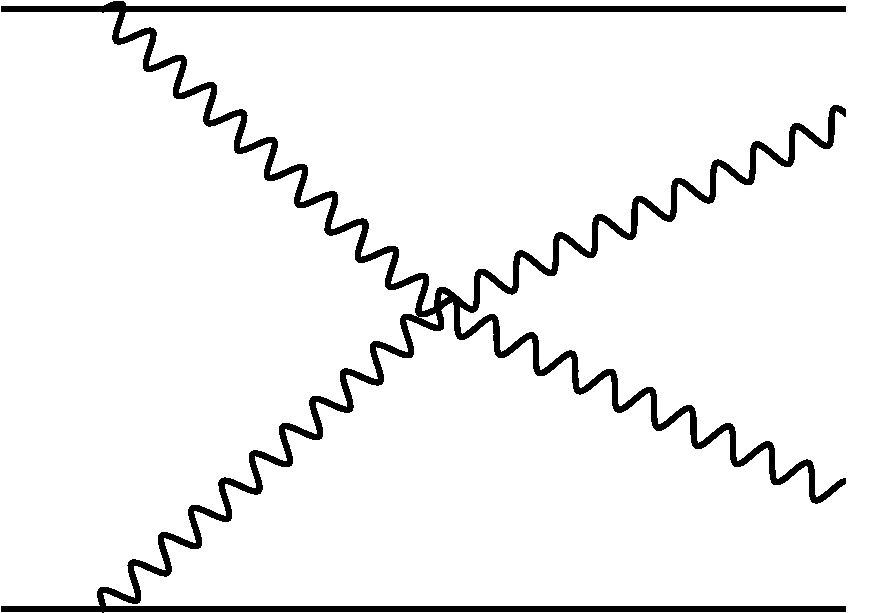
\includegraphics[width=0.3\textwidth,keepaspectratio]{figures/samples/feynVBS2.pdf}
}
\subfigure[]{
 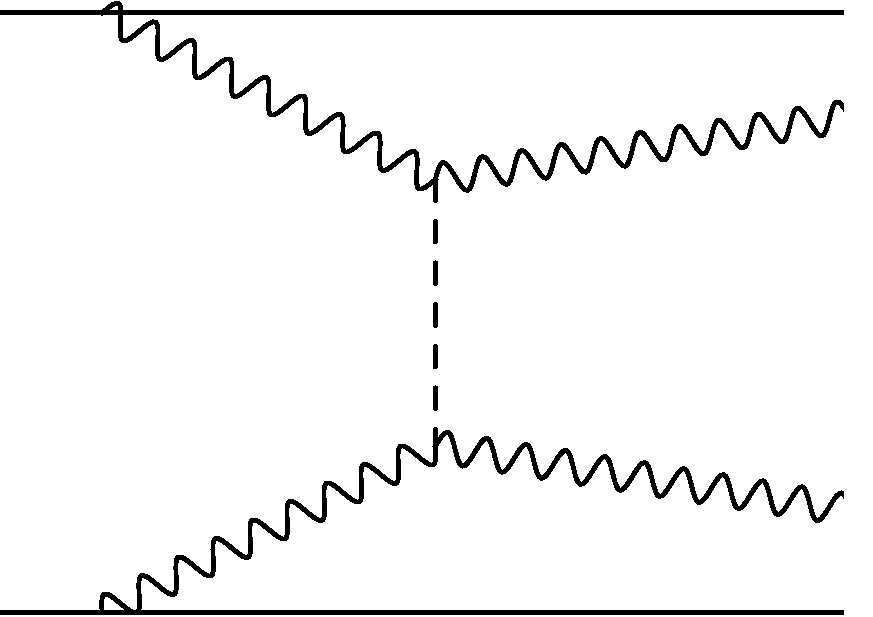
\includegraphics[width=0.3\textwidth,keepaspectratio]{figures/samples/feynVBS1.pdf}
}
\subfigure[]{
 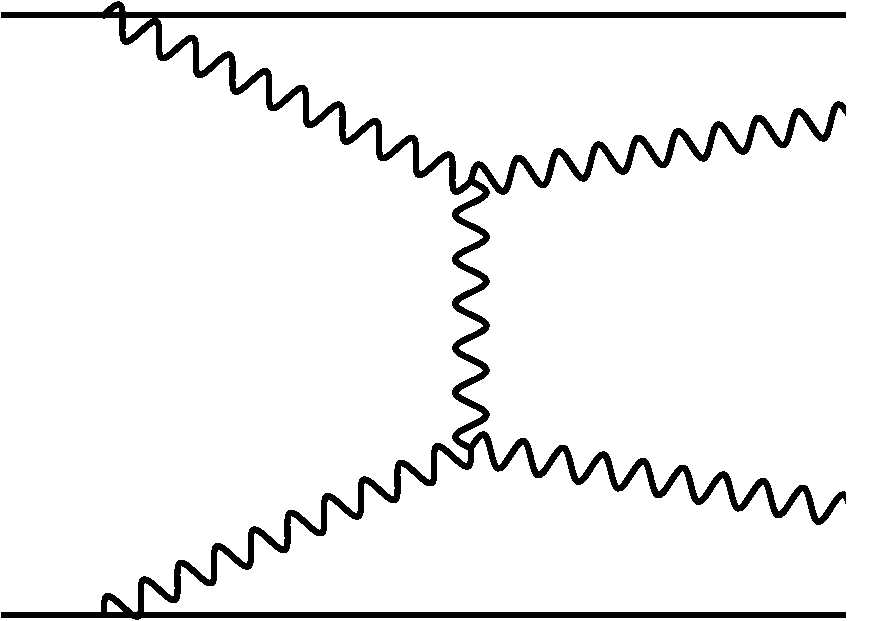
\includegraphics[width=0.3\textwidth,keepaspectratio]{figures/samples/feynVBS3.pdf}
}
\subfigure[]{
 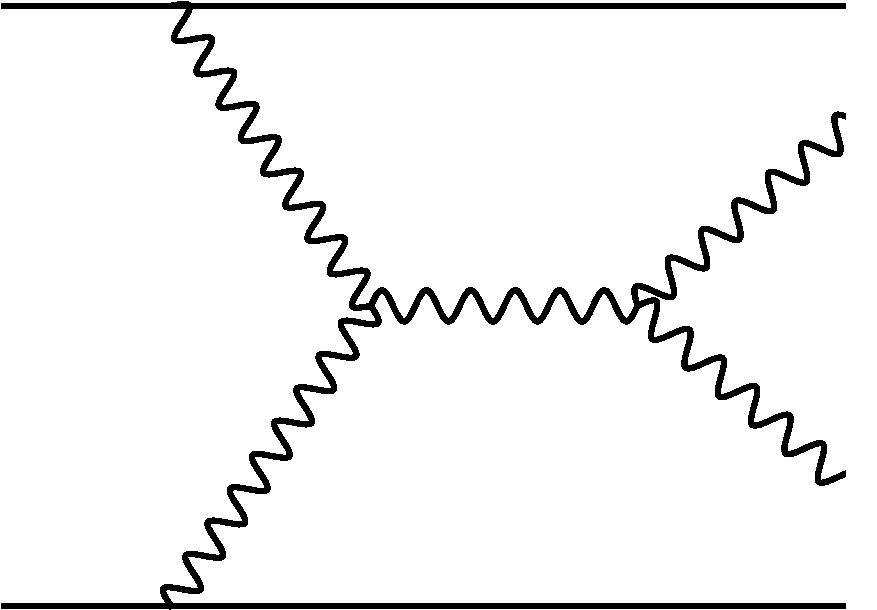
\includegraphics[width=0.3\textwidth,keepaspectratio]{figures/samples/feynVBS4.pdf}
}
\subfigure[]{
 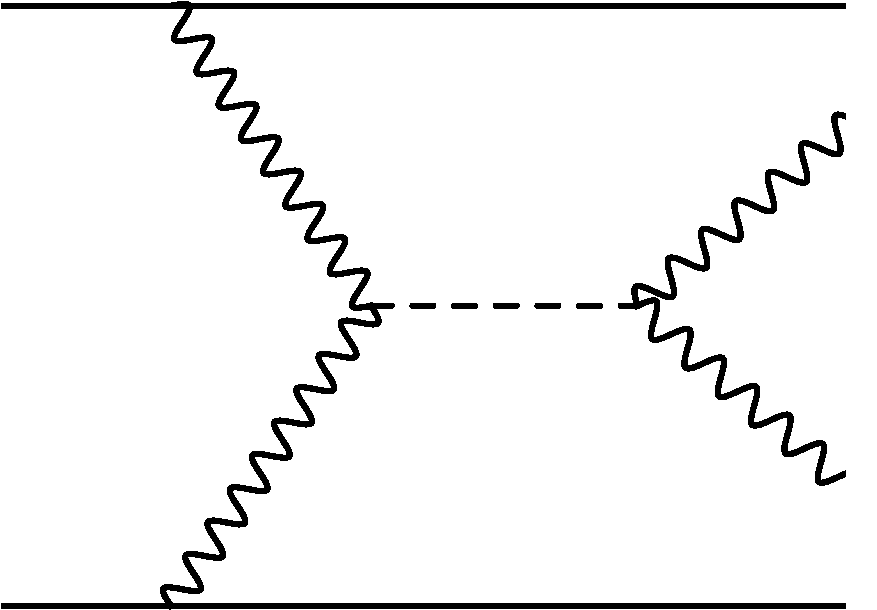
\includegraphics[width=0.3\textwidth,keepaspectratio]{figures/samples/feynVBS5.pdf}
}
\caption{
Examples of VBS diagrams that contribute to the signal.  Note that not all VBS diagrams contain quartic gauge couplings.
The dashed line represents the Higgs boson.  These and other Feynman diagrams in this note are made
using the JaxoDraw~\cite{Binosi:2003yf} program. The decays of the bosons are not shown.
}
\label{fig:feynmanVBS}
\end{center}
\end{figure}

%% feynman diagrams, non-VBS
%
\begin{figure}[tbp]
\begin{center}
\subfigure[]{
 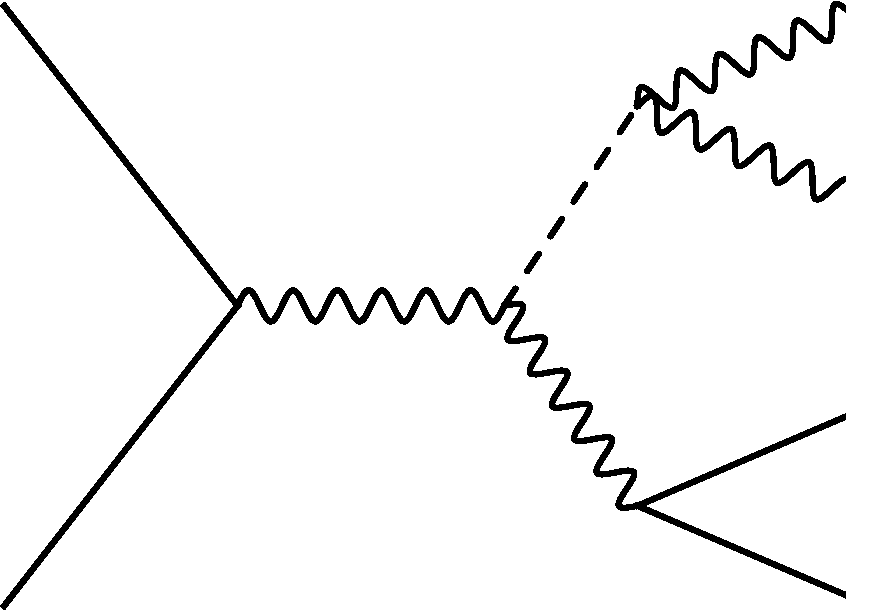
\includegraphics[width=0.3\textwidth,keepaspectratio]{figures/samples/feynEWKnonVBS3.pdf}
}
\subfigure[\label{subfig:feynEWKnonVBSb}]{
 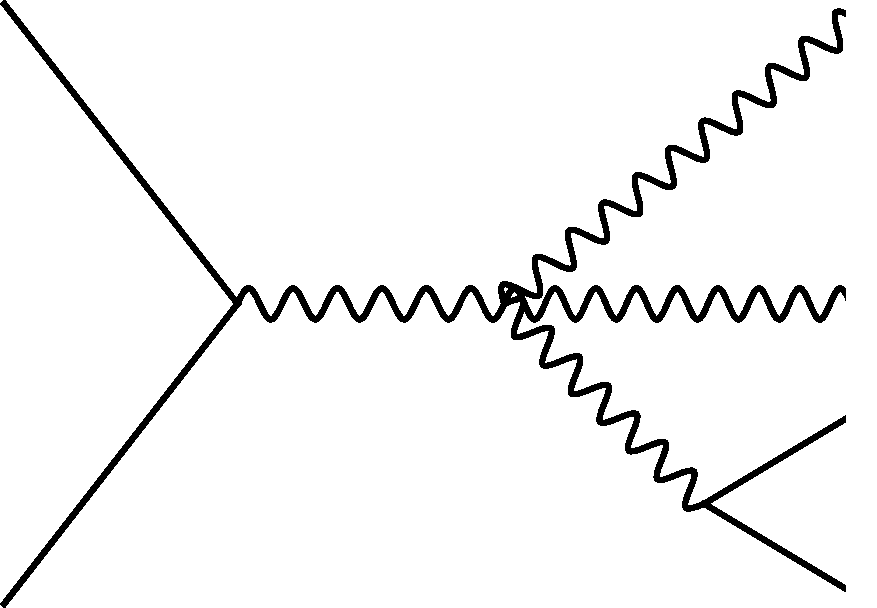
\includegraphics[width=0.3\textwidth,keepaspectratio]{figures/samples/feynEWKnonVBS4.pdf}
}
\subfigure[]{
 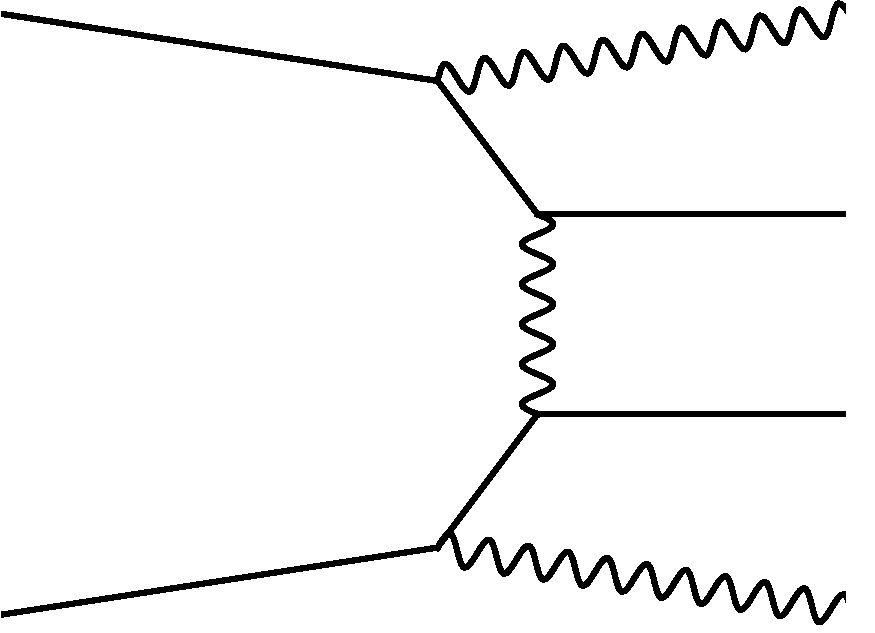
\includegraphics[width=0.3\textwidth,keepaspectratio]{figures/samples/feynEWKnonVBS5.pdf}
}
\subfigure[]{
 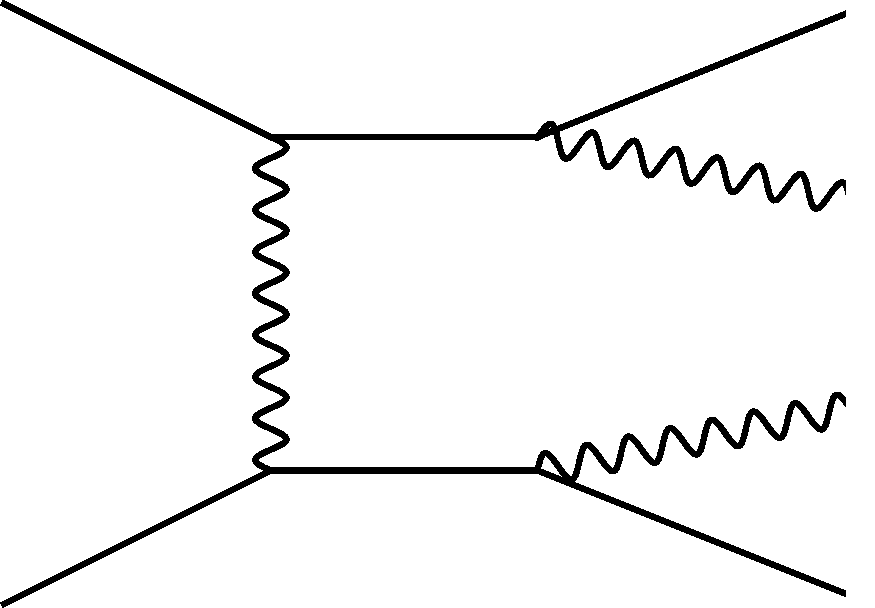
\includegraphics[width=0.3\textwidth,keepaspectratio]{figures/samples/feynEWKnonVBS6.pdf}
}
\subfigure[]{
 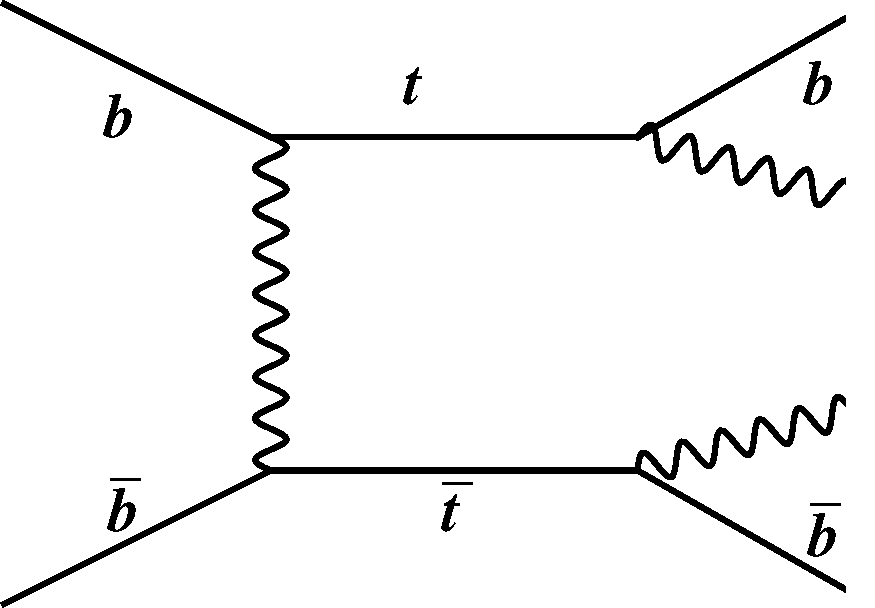
\includegraphics[width=0.3\textwidth,keepaspectratio]{figures/samples/feynEWKnonVBS1.pdf}
}
\subfigure[]{
 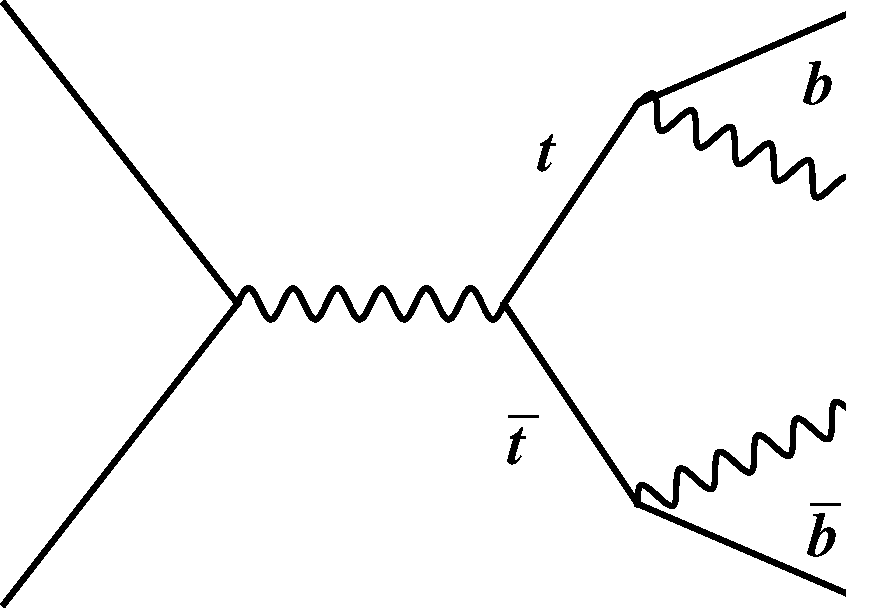
\includegraphics[width=0.3\textwidth,keepaspectratio]{figures/samples/feynEWKnonVBS2.pdf}
}
\subfigure[]{
 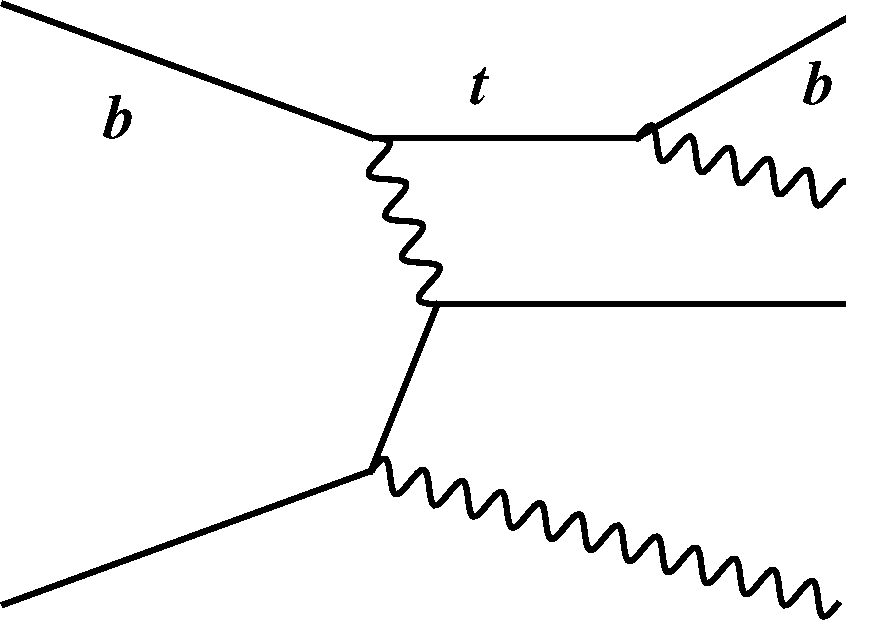
\includegraphics[width=0.3\textwidth,keepaspectratio]{figures/samples/feynEWKnonVBS7.pdf}
}
\caption{
Examples of non-VBS $\mathcal{O}(\alpha_{EW}^6)$ diagrams that contribute to the signal. The decays of the bosons are not
explicitly shown, but the counting of powers of $\alpha$ includes the boson decays.
}
\label{fig:feynmanEWKnonVBS}
\end{center}
\end{figure}

%% feynman diagram, tZb
\begin{figure}[tbp]
\begin{center}
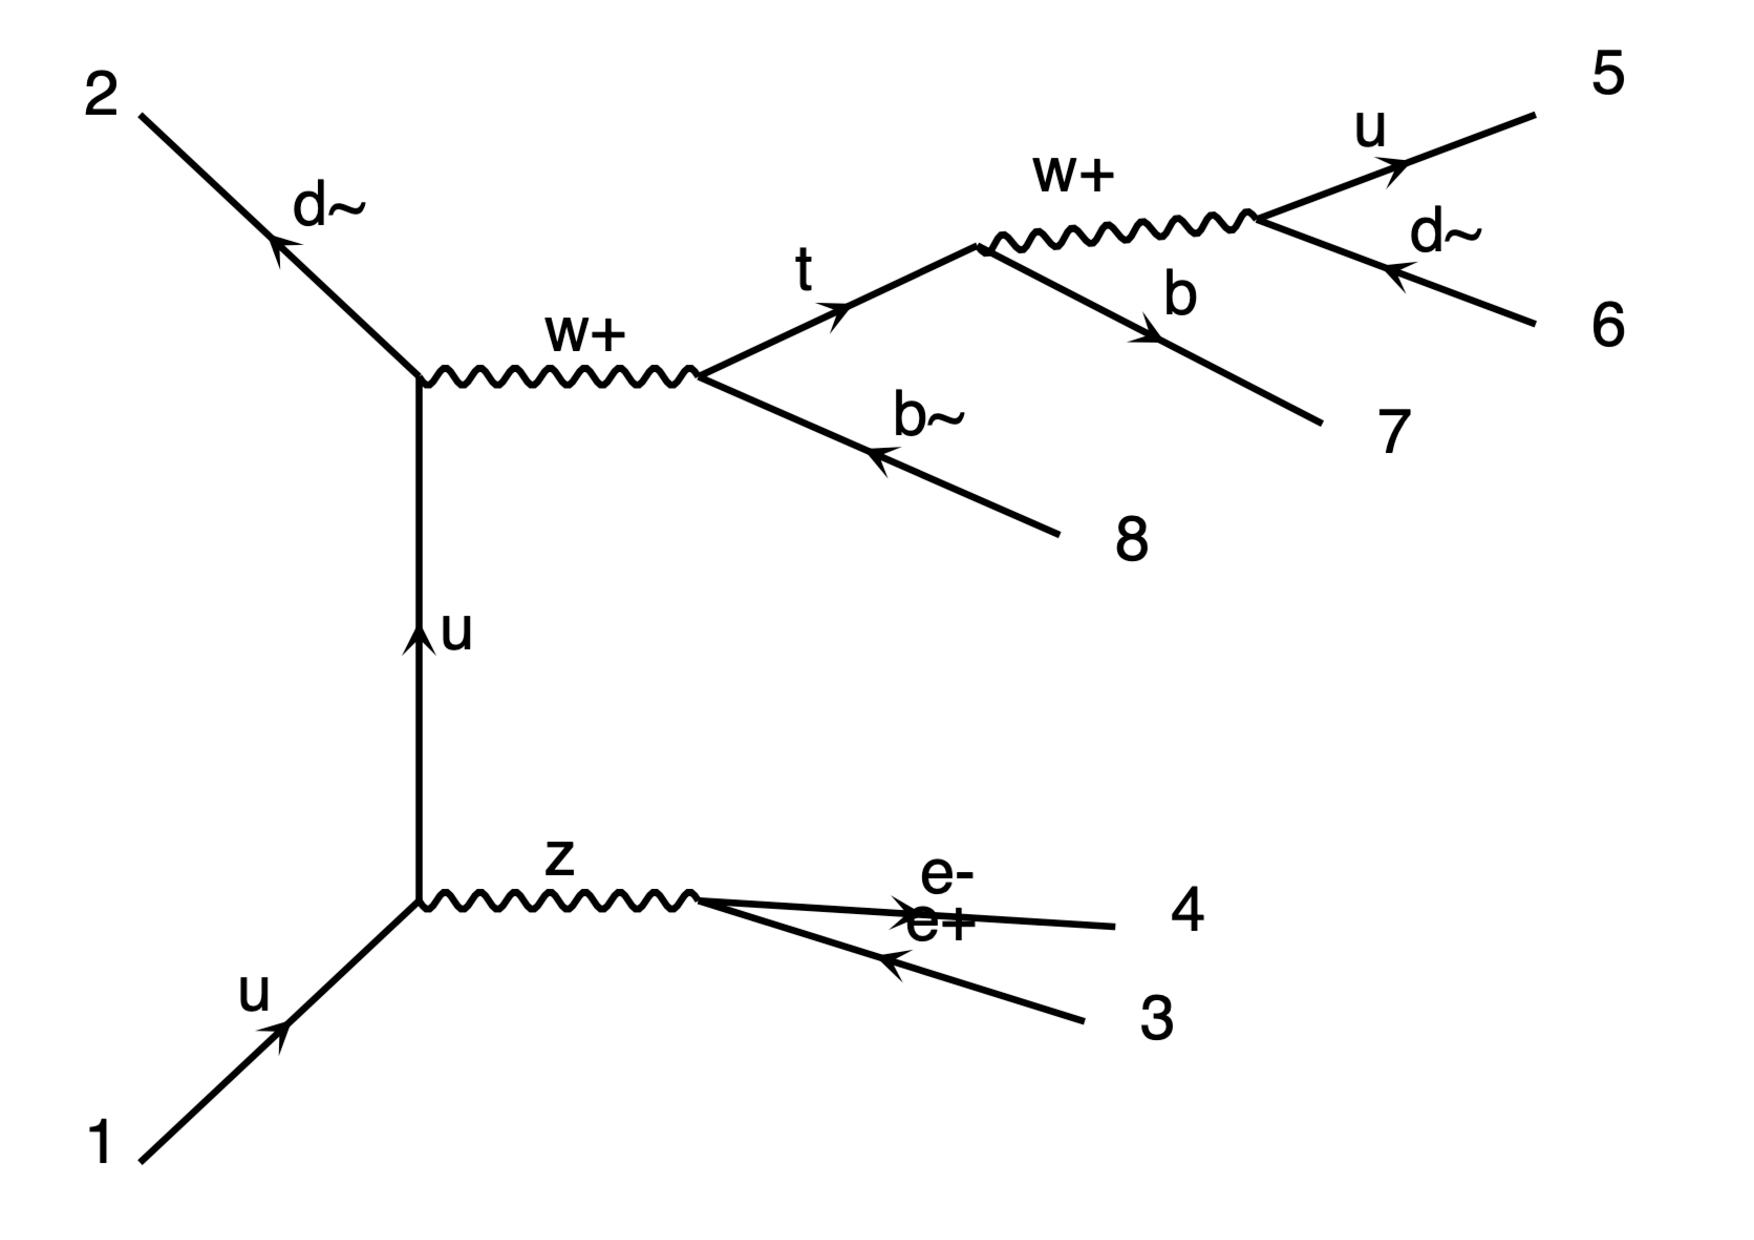
\includegraphics[width=0.3\textwidth,keepaspectratio]{figures/samples/feynEWKnonVBStZb.pdf}
\caption{
The example of the tZb diagram, which included in non-VBS $\mathcal{O}(\alpha_{EW}^6)$ diagrams.
}
\label{fig:feynmantZb}
\end{center}
\end{figure}

%% feynman diagrams, QCD
%
\begin{figure}[tbp]
\begin{center}
\subfigure[]{
 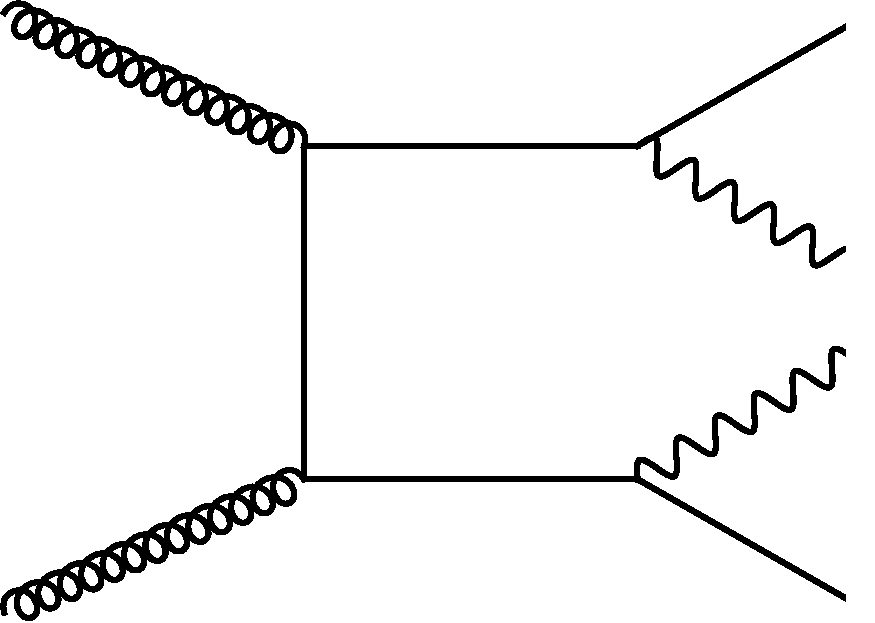
\includegraphics[width=0.3\textwidth,keepaspectratio]{figures/samples/feynQCD3.pdf}
}
\subfigure[]{
 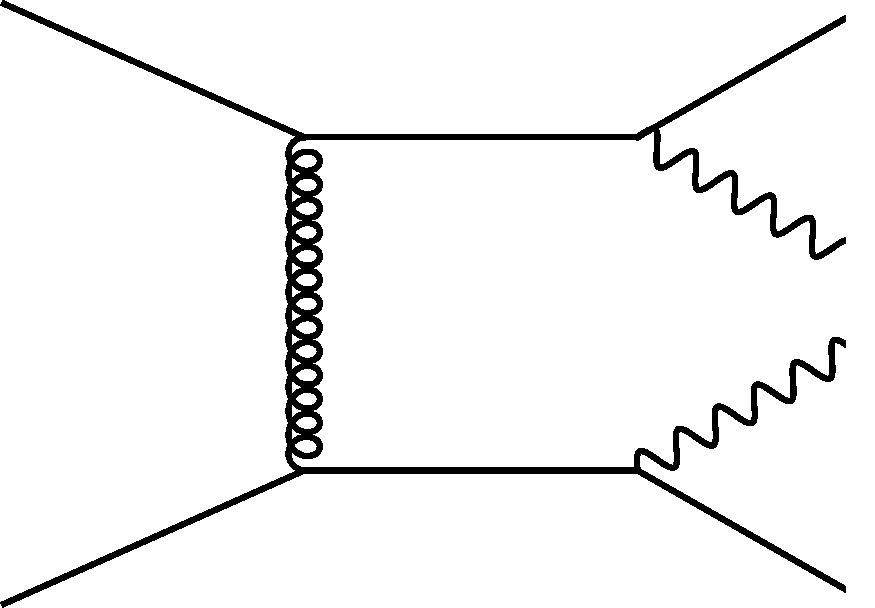
\includegraphics[width=0.3\textwidth,keepaspectratio]{figures/samples/feynQCD4.pdf}
}
\subfigure[]{
 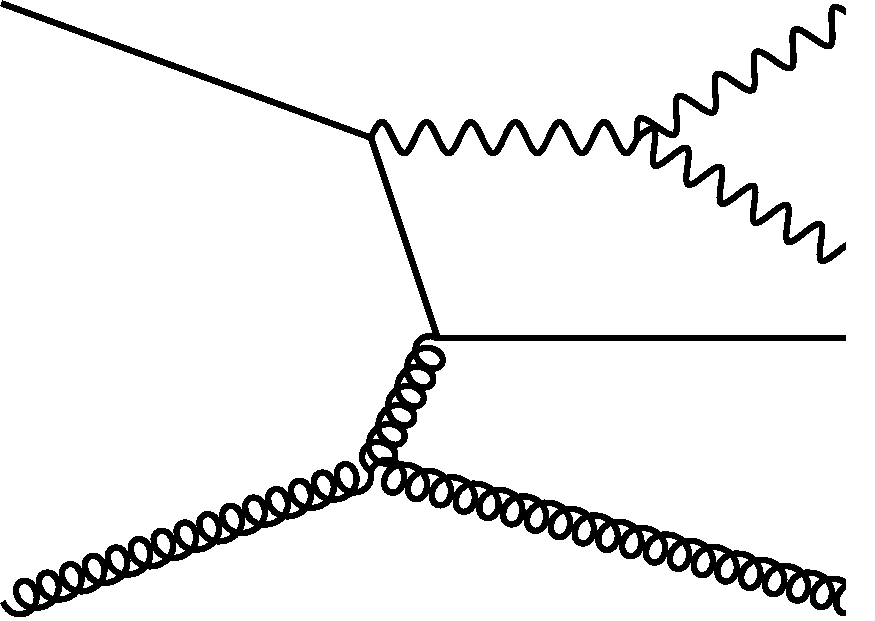
\includegraphics[width=0.3\textwidth,keepaspectratio]{figures/samples/feynQCD5.pdf}
}
\subfigure[]{
 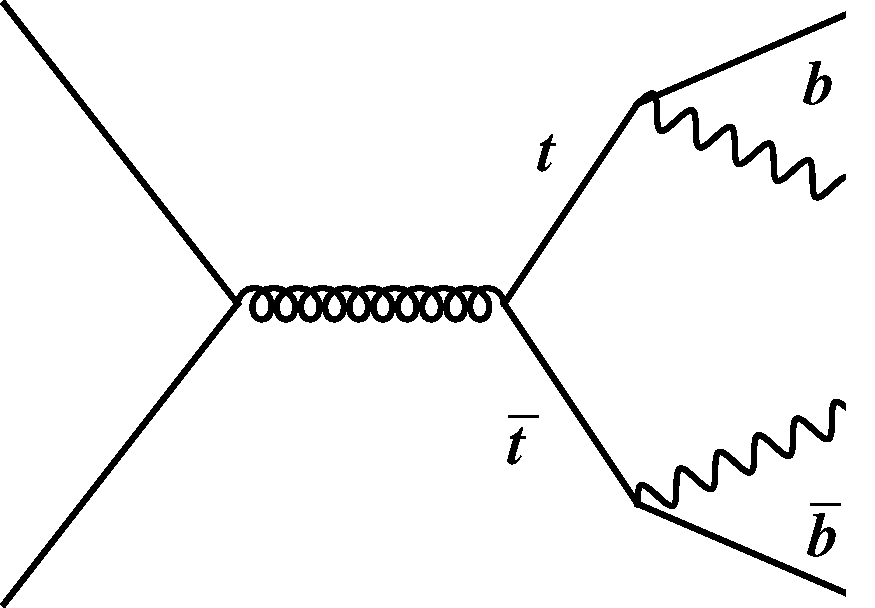
\includegraphics[width=0.3\textwidth,keepaspectratio]{figures/samples/feynQCD1.pdf}
}
\subfigure[]{
 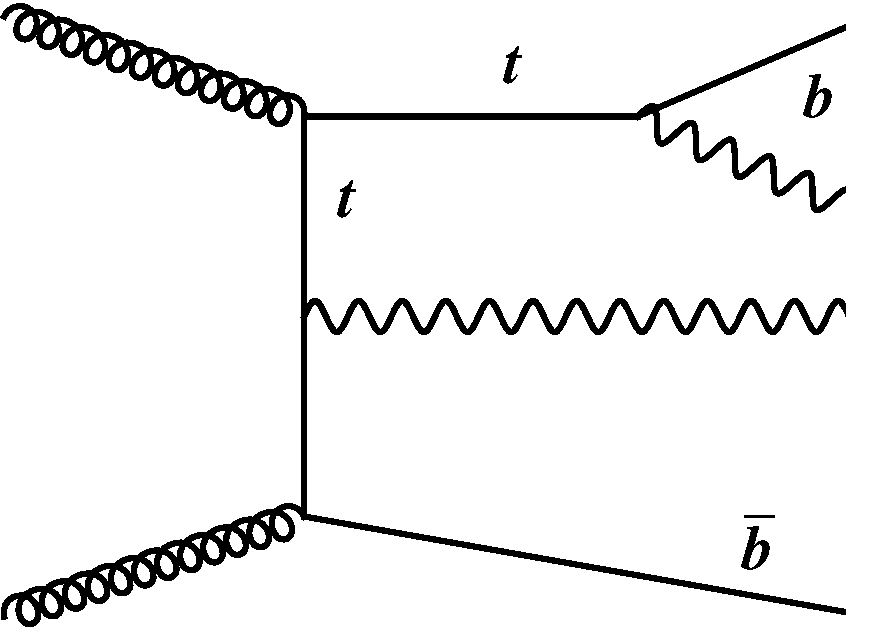
\includegraphics[width=0.3\textwidth,keepaspectratio]{figures/samples/feynQCD2.pdf}
}
\caption{
Examples of $\mathcal{O}(\alpha_{EW}^4 \alpha_{S}^2)$ diagrams that lead to the $VV$+2parton final state. These
are not included in the signal definition.  The decays of the bosons are not
explicitly shown, but the counting of powers of $\alpha$ includes the boson decays.
}
\label{fig:feynmanQCD}
\end{center}
\end{figure}



\section{Anomalous Quartic Gauge Coupling and Effective Field Theory}

To model possible aQGC effect in the VBS process, the Eboli model \cite{eboli2006p} which introduces 21 new dim-8 operators which satisfy the SM $SU(2)\times U(1)_Y$ symmetry is used.
Of these operators, 19 can effect the semileptonic VBS final state.
As typical for EFT expansions, the modified lagrangian with these new operators $\mathcal{L}_n$ and corresponding Wilson coeffiencts $c_n$ and UV scale $\Lambda$ is:
\begin{equation*}
  \mathcal{L}=\mathcal{L}_{sm}+\sum_{n}\frac{c_n}{\Lambda^{4}}\mathcal{L}_n
\end{equation*}

In generality, the matrix-element of a SM process with the addition of new EFT contributions can be written as:
\begin{equation}
  |A_{SM}+c_iA_i|=|A_{SM}^2|+\sum\limits_i c_i^2|A_{i}^2|+ \sum\limits_i 2 c_i \mathrm{Re}(A_{SM}^\star A_i) +\sum\limits_{i\neq j} c_i c_j \mathrm{Re}(A_i^\star A_j)
\end{equation}
where $|A_SM|^2$ is the SM matrix element, $|A_{i}^2|$ represents the pure-EFT matrix element, $2 \mathrm{Re}(A_{SM}^\star A_i)$ is their corresponding interference term, and $\mathrm{Re}(A_i^\star A_j)$ is the possible interference between EFT amplitudes.
This structure can be exploited in recent MadGraph5\_aMC@NLO versions which allows the specific generation of each of these terms individually, known as the matrix-element decomposition method.

Typically one would need to generate a series of samples for each operator $A_i$ at different $c_i$ values, to derive a series of template functions for $|A_{SM}+c_iA_i|$ which would need to be interpolated between for arbitrary $c_i$. Generating samples with the decomposition method greatly simplifies this procedure as one only now needs to generate for each operator $A_i$ the corresponding pure-EFT and interference terms (as well as cross-interference terms if needed). These templates can then be scaled either quadratically or linear with the corresponding $c_i$ values to generate the required full template $|A_{SM}+c_iA_i|$.

The Eboli dim-8 EFT processes are modeled using MadGraph5\_aMC@NLO v2.7.2~\cite{Alwall:2014hca} at LO with the  \textsc{NNPDF30LO} PDF set~\cite{Ball:2012cx} plus \PYTHIA8.244~\cite{Sjostrand:2007gs} for fragmentation.
The matrix-element calculation produces two on-shell $W/Z$ bosons, which are subsequently decayed with \textsc{Madspin}~\cite{Artoisenet:2012st} to simulate the leptonic and hadronic decays of the bosons.
The use of Madspin is required for use of the matrix-element weighting and requires separate generation for each weak isospin state of the boson (i.e the following processes are simulated separately: $W^+W^-$, $W^+W^+$, $W^-W^-$, $W^+Z$, $W^-Z$, $ZZ$).
Each of the 19 contributing operators, across the 6 intermediate diboson state processes and 3 final semileptonic final state processes are generated separately for the pure-BSM and interference term.



